% Largement inspiré par l'excellent exemple français de présentation de Till Tantau (2004) et Philippe de Sousa (2006) : https://github.com/josephwright/beamer/blob/master/doc/solutions/conference-talks/conference-ornate-20min.fr.tex

\usepackage{lmodern}
\usepackage[french]{babel}
\usepackage[utf8]{inputenc}
\usepackage[T1]{fontenc}

\setbeamertemplate{caption}{\raggedright\insertcaption\par} % Suppression du Figure ou Table préfixé dans les \caption par beamer :  https://tex.stackexchange.com/a/82460

\mode<presentation> {
  \usetheme{default}
  \useinnertheme{circles}
  \useoutertheme[subsections=false]{smoothbars}
  \usecolortheme[rgb={0.8,0,0}]{structure}
}

\AtBeginSection[] {
  \begin{frame}<beamer>{Plan de la soutenance}
    \tableofcontents[currentsection]
  \end{frame}
}

\title{Agrandissement d'un écran mobile par réalité augmentée}
\author{Erwan Normand}
\institute{Soutenance de mémoire de maîtrise}
\date{\frenchdate{2018}{08}{29}}

\newcommand{\twocols}[2]{% Side-By-Side colums
  \begin{columns}%
    \begin{column}{0.5\textwidth}#1\end{column}%
    \begin{column}{0.5\textwidth}#2\end{column}%
  \end{columns}%
}
\newcommand{\figuregraphic}[2][1]{%
  \includegraphics[width=#1\textwidth, height=5cm, keepaspectratio]{figures/#2}%
}
\newcommand{\figurecaption}[3][1]{%
  \begin{figure}%
    \figuregraphic[#1]{#2}
    \caption{#3}%
  \end{figure}%
}

\begin{document}

\frame{\maketitle}

\begin{frame}{Plan de la soutenance}
  \tableofcontents
\end{frame}

\section{Problématique}

\begin{frame}{La réalité augmentée (RA)}
  \twocols{
    \begin{itemize}[<+->]
      \item Définition : contenu virtuel inséré dans l'environnement réel.
      \item Avancées techniques en 2016/2017 : HoloLens, ARKit, ARCore.
      \item Usages très prometteurs.
      \item Les interfaces humain-machine en RA sont peu maîtrisées.
    \end{itemize}
  }{
    \only<1>{\figurecaption{MobileAR}{Application de RA sur téléphone [Wikipedia]}}
    \only<2>{\figurecaption{HoloLens_1}{Publicité du visiocasque HoloLens [Microsoft]}}
    \only<3>{\figurecaption{HoloLens_2}{Skype sur le HoloLens [Microsoft]}}
    \only<4>{\figurecaption{UnityFutureMRPartIII2017}{Bureau de travail en RA [Unity]}}
  }
\end{frame}

\begin{frame}{Les interfaces humain-machine (IHM)}
  \twocols{
    \begin{itemize}[<+->]
      \item IHM : interface d'un utilisateur avec un ordinateur.
      \item Trouver les techniques d'interactions les plus adaptées.
      \item Réduire l'écart entre entrées et sorties.
    \end{itemize}
  }{
    \figurecaption{Billinghurst2005}{Principe d'une IHM \cite{Billinghurst2005}}
  }
\end{frame}

\begin{frame}{IHM pour la RA}
  \twocols{
    \begin{itemize}
      \item<1-> La RA permettrait de fondre l'ordinateur dans l'environnement.
      \item<2-> Mais encore aucun paradigme d'IHM pour la RA.
      \item<3-> Difficile car entrées \alert{et} sorties sont en 3D.
      \item<4-> Techniques d'interactions courantes :
      \begin{itemize}
        \item Main virtuelle
        \item<5-> Pointeur virtuel
      \end{itemize}
    \end{itemize}
  }{
    \only<1-2>{\figurecaption{Serrano2015_1}{Gluey \cite{Serrano2015}}}
    \only<3>{\figurecaption{Lee2013}{SpaceTop \cite{Lee2013}}}
    \only<4>{\figurecaption{Taylor2016}{Main virtuelle \cite{Taylor2016}}}
    \only<5>{\figurecaption{Pfeuffer2017_1}{Pointeur virtuel \cite{Pfeuffer2017}}}
  }
\end{frame}

\begin{frame}{Augmenter un téléphone par RA}
  \twocols{
    \begin{itemize}[<+->]
      \item Les téléphones ont une taille limitée pour être tenu en main.
      \item Un plus grand écran serait utile.
      \item Les interactions tactiles sont précises et connues.
      \item Des interactions sur un écran virtuel pourraient être intuives mais difficiles.
    \end{itemize}
  }{
    \only<1,3>{\figurecaption{Heun2016}{Reality Editor \cite{Heun2016}}}
    \only<2>{\figurecaption{Baudisch2002}{Écran agrandi \cite{Baudisch2002}}}
    \only<4>{\figurecaption{LeapMotion2018_3}{Visiocasque de RA North Star [LeapMotion]}}
  }
\end{frame}

\begin{frame}{Problématique}
  \begin{block}<1->{}
     Est-ce qu’un téléphone à écran étendu donne un avantage à un utilisateur par rapport à un téléphone non-étendu ?
  \end{block}
  \begin{block}<2->{}
    Est-il préférable d’interagir avec une main virtuelle directement sur l’écran virtuel, autour du téléphone, ou en utilisant seulement l’écran tactile ?
  \end{block}
\end{frame}
\section{Concept} % Chapitre du concept
\begin{frame}{Titre}
  \begin{figure}
    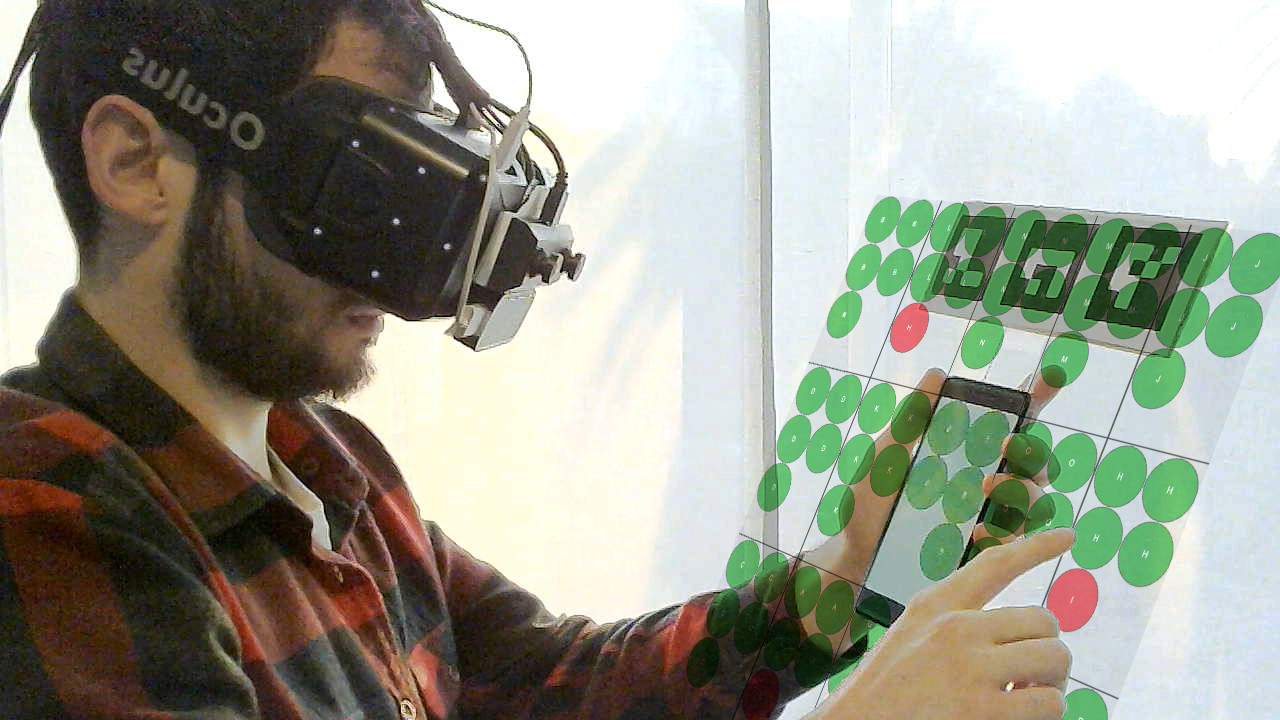
\includegraphics[height=6cm]{figures/HandheldVESADMidAirInArOut}
    \caption{Photomontage de notre prototype.}
  \end{figure}
\end{frame}
\section{Prototype}

\begin{frame}{Titre}
  contenu
\end{frame}
\section{Étude expérimentale}

\begin{frame}{Titre}
  contenu
\end{frame}
\section{Discussion}

\begin{frame}{Titre}
  contenu
\end{frame}
\section{Conclusion}

\begin{frame}{Conclusion}
\end{frame}

\appendix
\section<presentation>*{\appendixname}
\begin{frame}[allowframebreaks]{Bibliographie}
  \begin{thebibliography}{10}
    \bibitem[Billinghurst2005]{Billinghurst2005}
      Mark Billinghurst, Raphael Grasset, Julian Looser.
      \newblock Designing augmented reality interfaces.
      \newblock ACM SIGGRAPH Computer Graphics, 39(1), 17-22.

    \bibitem[Ens2014]{Ens2014}
      Barrett M. Ens, Rory Finnegan, Pourang P. Irani.
      \newblock The personal cockpit: A spatial interface for effective task switching on head-worn displays.
      \newblock CHI 2014.

    \bibitem[Grubert2015]{Grubert2015}
      Jens Grubert, Matthias Heinisch, Aaron J. Quigley, Dieter Schmalstieg.
      \newblock MultiFi: Multi fidelity interaction with displays on and around the body.
      \newblock CHI 2015.

    \bibitem[Heun2016]{Heun2016}
      Valentin Heun, James Hobin, Pattie Maes.
      \newblock Reality Editor: Programming Smarter Objects.
      \newblock UbiComp 2013.

    \bibitem[Lee2013]{Lee2013}
      Jinh Lee, Alex Olwal, Hiroshi Ishii, Cati Boulanger.
      \newblock SpaceTop: Integrating 2D and spatial 3D interactions in a see-through desktop environment.
      \newblock CHI 2013.

    \bibitem[Piumsomboon2013]{Piumsomboon2013}
      Thammathip Piumsomboon, Adrian Clark, Mark Billinghurst, Andy Cockburn.
      \newblock User-defined gestures for augmented reality.
      \newblock CHI 2013.

    \bibitem[Pfeuffer2017]{Pfeuffer2017}
      Ken Pfeuffer, Benedikt Mayer, Diako Mardanbegi, Hans Gellersen.
      \newblock Gaze + pinch interaction in virtual reality.
      \newblock UIST 2017.

    \bibitem[Serrano2015]{Serrano2015}
      Marcos Serrano, Barrett Ens, Xing-Dong Yang, Pourang Irani.
      \newblock Gluey: Developing a head-worn display interface to unify the interaction experience in distributed display environments.
      \newblock MobileHCI 2015.

    \bibitem[Serrano2015a]{Serrano2015a}
      Marcos Serrano, Barrett Ens, Xing-Dong Yang, Pourang Irani.
      \newblock Desktop-Gluey: Augmenting desktop environments with wearable devices.
      \newblock MobileHCI 2015.

    \bibitem[Taylor2016]{Taylor2016}
      Jonathan Taylor, Lucas Bordeaux, Thomas J. Cashman, Bob Corish, Cem Keskin, Toby Sharp, Eduardo Soto, David Sweeney, Julien P. C. Valentin, Benjamin Luff, Arran Topalian, Erroll Wood, Sameh Khamis, Pushmeet Kohli, Shahram Izadi, Richard Banks, Andrew W. Fitzgibbon, Jamie Shotton.
      \newblock Efficient and precise interactive hand tracking through joint, continuous optimization of pose and correspondences.
      \newblock ACM Transactions on Graphics, 35(4), 1-12.

    \bibitem[Wobbrock2009]{Wobbrock2009}
      Jacob O. Wobbrock and Meredith Ringel Morris and Andrew D. Wilson.
      \newblock User-defined gestures for surface computing.
      \newblock CHI 2009.
  \end{thebibliography}
\end{frame}

\end{document}